\documentclass[12pt]{article}
\usepackage{amsmath}
\usepackage{amssymb}
\usepackage{amsthm}
\usepackage{amsfonts}
\usepackage{graphicx} 
\usepackage{amsthm}
\graphicspath{{./img/}}

\title{Homework 10\
\\11.2-11.4}
\author{Rafael Betita\\
MATH 005BH - Single Variable Calculus II}
\date{November 1, 2018}

\begin{document}
\maketitle

\newpage\section{Definitions}
\begin{enumerate}
    \item\begin{enumerate}
        \item What is the difference between a sequence and a series? 
        \\\\A sequence is a list of numbers written in a definite order. A series is typically known to be the sum of the terms of a sequence. 
        \\
        \item What is a convergent series? A divergent series?
        \\\\ A convergent series is an infinite sequence which a finite sum, while a divergent series has no finite sum and instead has a sum that diverges onto infinity
        \\
        \item An infinite series converges if its sum or limit is a finite number.
    \end{enumerate}
    \item Explain what it means to say $\sum^\infty_{n=1}a_n=5$
    \\\\ This expression is basically saying that as $n$ approaches infinity, the sum of the series $a_n$ approaches 5.
    \item 
    \begin{enumerate}
        \item $\sum_{n=1}^\infty\frac{1}{n^4+n^2}$ Converges
        \begin{align*}
            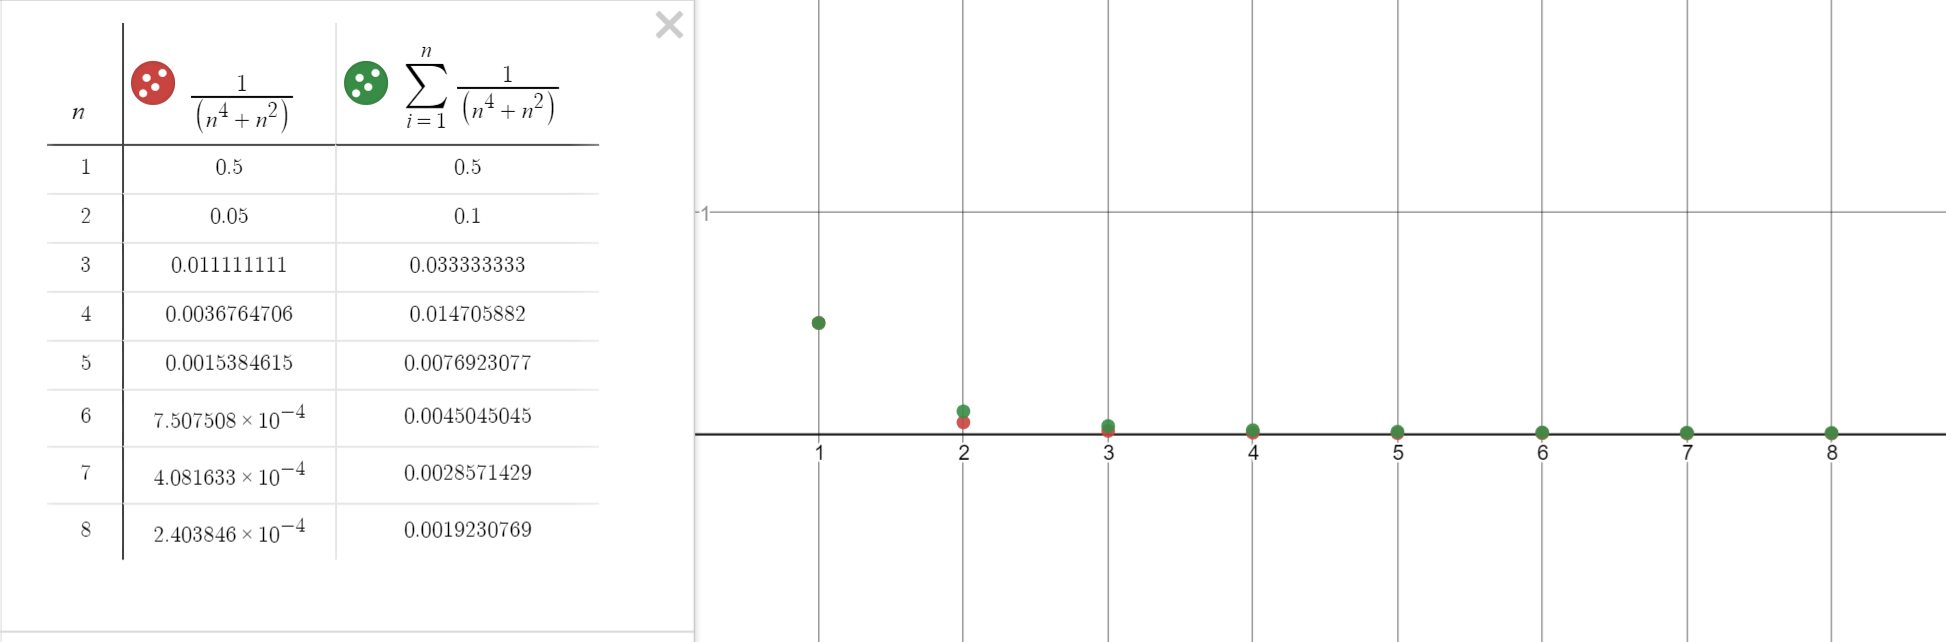
\includegraphics[width=\linewidth]{10_1}
        \end{align*}
        \newpage\item $\sum_{n=1}^\infty\frac{1}{\sqrt[3]{n}}$ Diverges
        \begin{align*}
            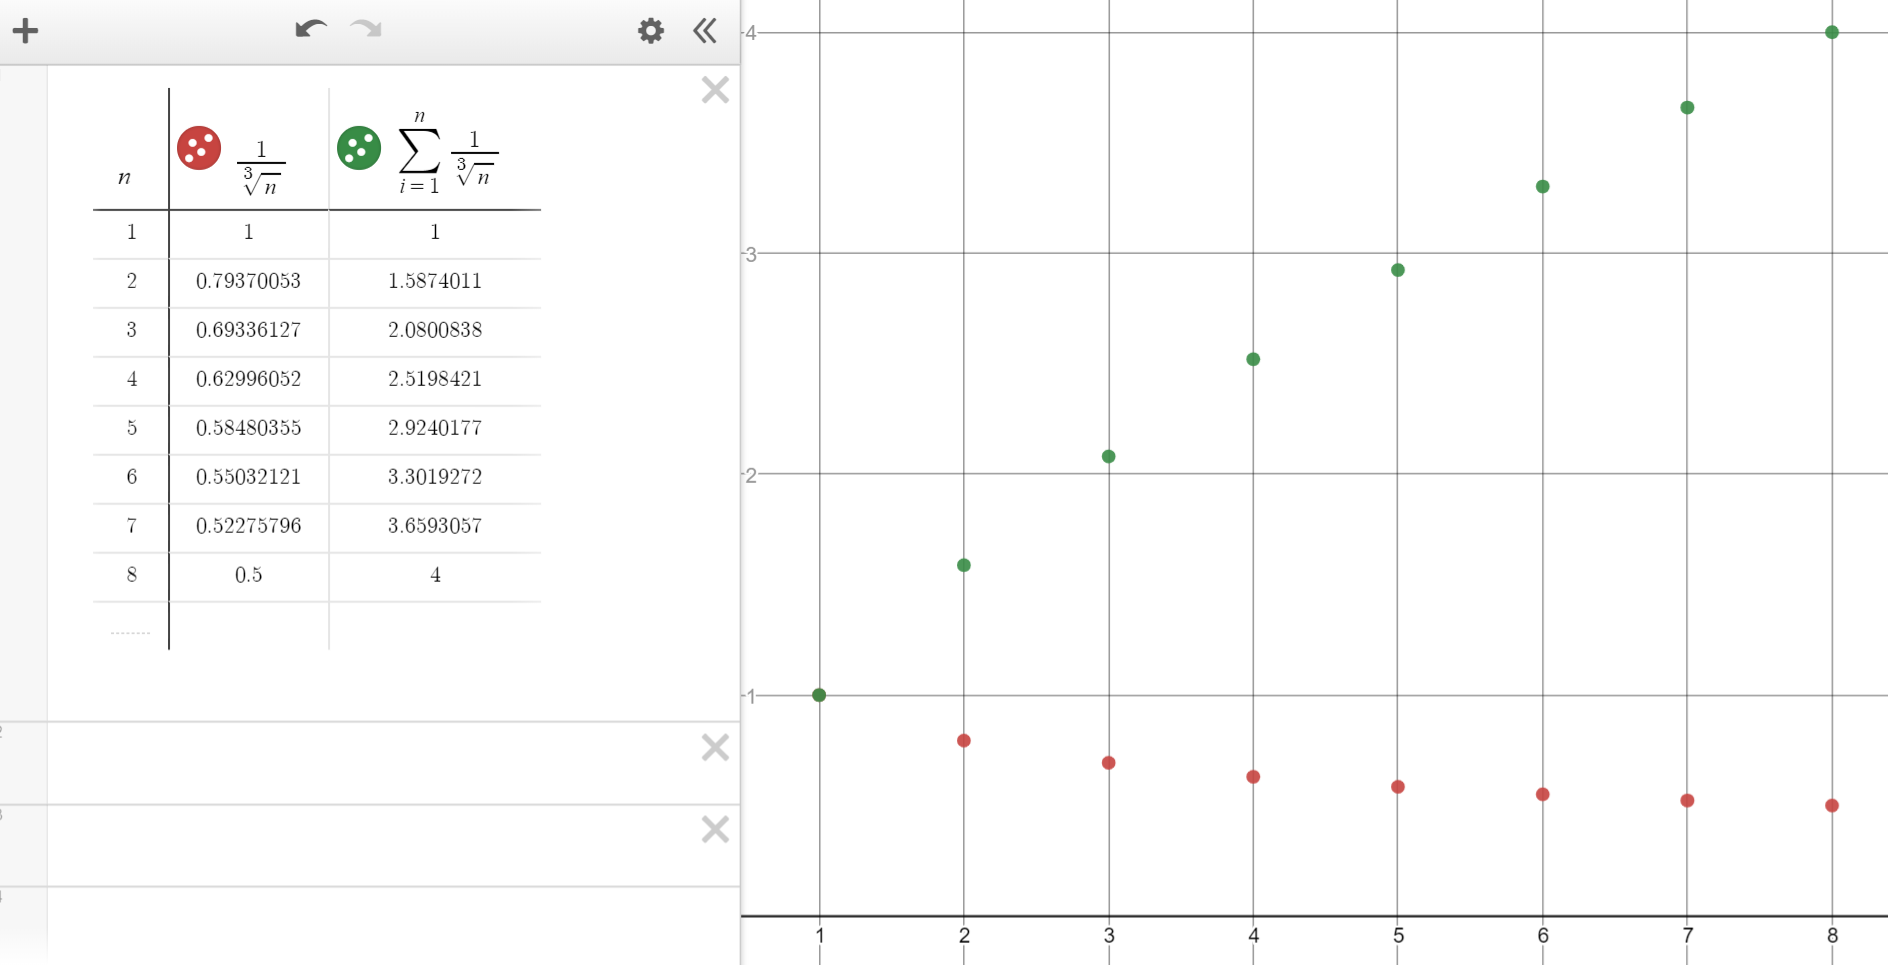
\includegraphics[width=\linewidth]{10_2}
        \end{align*}
    \end{enumerate}
    \item 
    \begin{enumerate}
        \item $\sum_{n=1}^\infty\frac{n}{\sqrt{n^2+4}}$
        \begin{align*}
            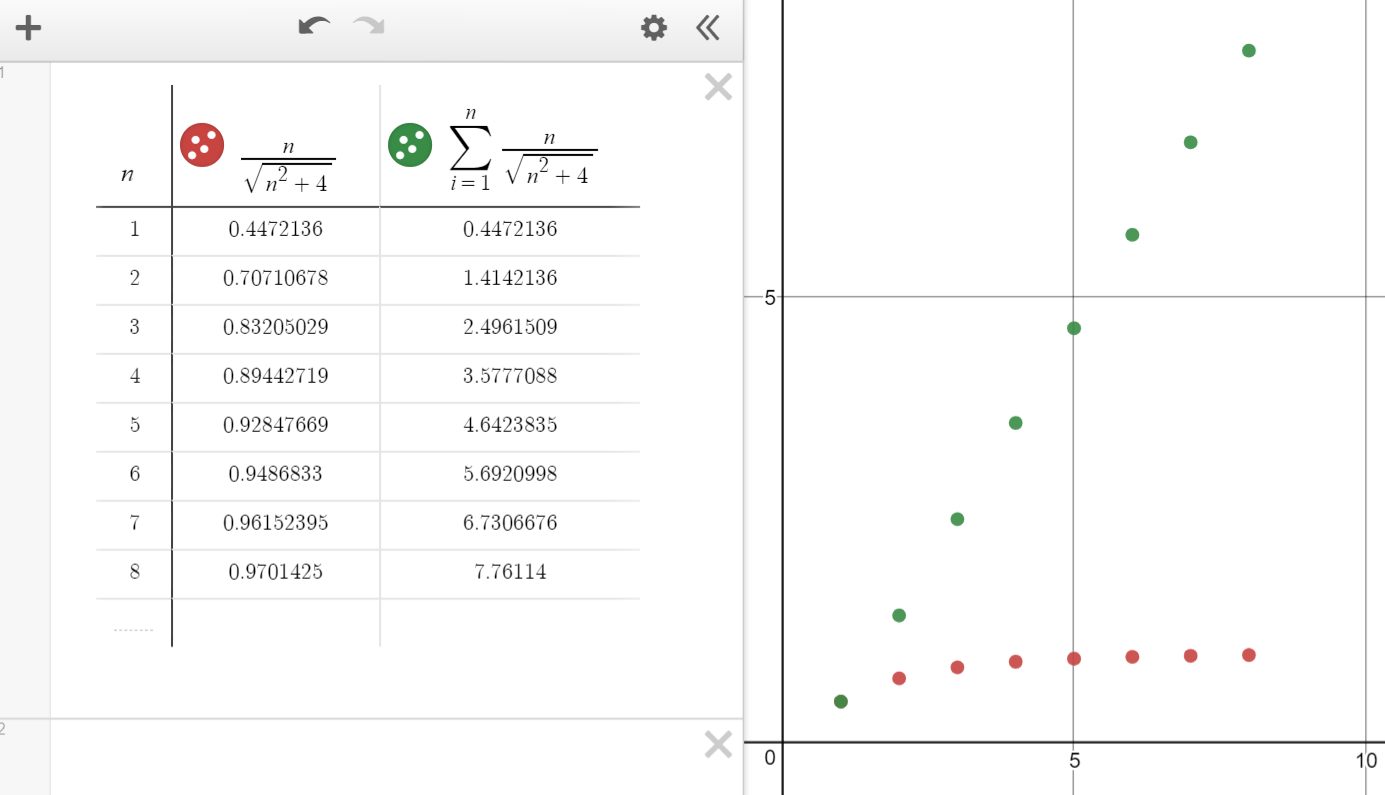
\includegraphics[width=\linewidth]{10_3}
        \end{align*}
    Graph appears to be divergent. This is because as the sequence grows, its result infinitely gets closer to 1. Therefore the series will infinitely grow in turn.
        \item $\sum_{n=1}^\infty\frac{7^{n+1}}{10^n}$
        \begin{align*}
            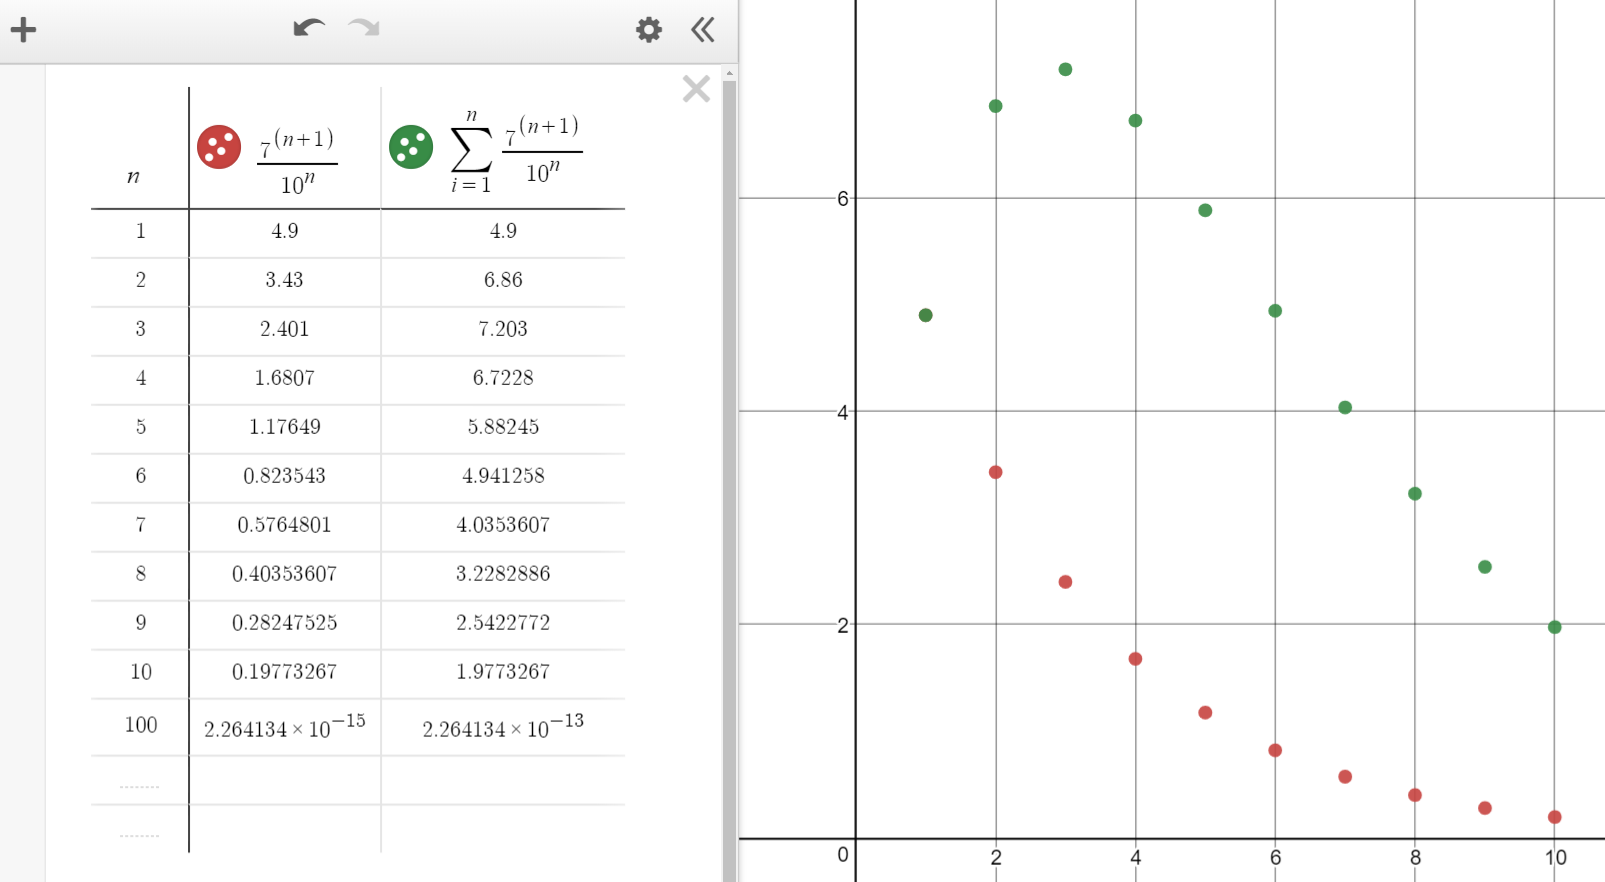
\includegraphics[width=\linewidth]{10_4}
        \end{align*}
        Graph appears to be convergent. We will need to calculate it manually. It looks to be a geometric series so we use the property of checking for the ratio and the constant. Where $a=7$ and $r=\frac{7}{10}$. We use property 4 as defined in page 750 where the sum can be found as $\frac{a}{1-r}$
        \begin{align*}
            \sum_{n=1}^\infty\frac{7^{n+1}}{10^n} \to \frac{7\cdot7^{n}}{10^n}\to\frac{7}{\frac{3}{10}}=\frac{70}{3}
        \end{align*}
    \end{enumerate}
    \item (11.2 15) Let $a_n = \frac{2n}{3n+1}$
    \begin{enumerate}
        \item Determine whether $\{a_n\}$ is convergent.
        \begin{align}
            \lim_{n\to\infty}\frac{2n}{3n+1}=\lim_{n\to\infty}\frac{2}{3+\frac{1}{n}}=\frac{2}{3}\to\text{ Convergent}
        \end{align}
        \item Determine whether $\sum_{n=1}^\infty$ is convergent.
        \\\\ Since our limit was found to be convergent to $\frac{2}{3}$ then our result follows the Divergence Test, where if $\lim_{n\to\infty}a_n\neq0$ or DNE then the series is divergent.
    \end{enumerate}
\end{enumerate}
\newpage\section{Series Where We Can Find the Sum}
    \subsection{Geometric Series}
    \begin{enumerate}
        \addtocounter{enumi}{5}\item How do you recognize that a series is geometric?
        \\\\ You can determine a series is geometric when each term is observed to be obtained from the preceding term. The first term in the series is called $a$. While the common ratio is often represented as $r$. The equation of a geometric series is as follows: $\sum^\infty_{n=1}ar^{n-1}$ where $a\neq 0$
        \item Determine if the following geometric series converge of diverge.
        \begin{enumerate}
            \item (11.2 17) 
            $3-4+\frac{16}{3}-\frac{64}{9}+...$
            \begin{align*}
                a=3 && r=-\frac{4}{3} && \text{$\left|-\frac{4}{3}\right|>1$ divergent series}
            \end{align*}
            \item (11.2 23) 
            $\sum_{n=1}^\infty\frac{(-3)^{n-1}}{4^n}$
            \begin{align*}
                r = \frac{(-3)^{-1}(-3)^{n}}{4^n}\to-\frac{3}{4}\\
                a_1 = \frac{(-3)^{1-1}}{4^1} = \frac{1}{4}\\
                \sum_{n=1}^\infty\frac{(-3)^{n-1}}{4^n}=\frac{\frac{1}{4}}{1+\frac{3}{4}}=\frac{1}{7} \text{ Convergent}
            \end{align*}
            \item (11.2 25)
            $\sum_{n=1}^\infty\frac{e^{2n}}{6^{n-1}}$
            \begin{align*}
                \sum_{n=1}^\infty\frac{(e^2)^{n}}{6^{-1}\cdot6^{n}} \text{where } r = \frac{e^2}{6} > 1 \text{ and is therefore divergent}
            \end{align*}
            \item (11.2 26)
            $\sum_{n=1}^\infty\frac{6\cdot2^{2n-1}}{3^n}$
            \begin{align*}
                r=\sum_{n=1}^\infty\frac{6\cdot2^{-1}\cdot(2^2)^n}{3^n}=\frac{4}{3} > 1 \text{ and is therefore divergent}
            \end{align*}
            \newpage\item (11.2 34)
                $\sum_{n=1}^\infty\frac{2^n+4^n}{e^n}$
            \begin{align*}
            \sum_{n=1}^\infty\frac{2^n+4^n}{e^n} = \sum_{n=1}^\infty\frac{2^n}{e^n} + \sum_{n=1}^\infty\frac{4^n}{e^n}\\
            r_1 = \frac{2}{e} < 1 \quad\quad\quad r_2 = \frac{4}{e} > 1
            \end{align*}
            $r_2$ is a divergent series therefore, $r$ is a divergent series
        \end{enumerate}
    \end{enumerate}
    \subsection{Telescoping Sum}
    \begin{enumerate}
        \addtocounter{enumi}{7}\item How do you recognize if a series is telescoping?
        \\\\When you add up its partial sums, the middle terms tend to cancel each other out, leaving the first and last terms as the sum. The sum "collapses" into just two terms, hence the name.
        \item Determine if the following series converge or diverge:
        \begin{enumerate}
            \item (11.2 47) $\sum^\infty_{n=1}(e^{\frac{1}{n}}-e^{\frac{1}{(n+1)}})$
            \begin{align*}
               \sum^\infty_{n=1}(e^{\frac{1}{n}}-e^{\frac{1}{(n+1)}})=(e^1-e^\frac{1}{2})+(e^\frac{1}{2}-e^\frac{1}{3}) + ...
            \end{align*}
           \text{Looks to be a telescoping series. We need to find sum the first and last term. }
            \begin{align*}
                \lim_{n\to\infty}(e^1-e^\frac{1}{n+1})=e-1 \text{  Convergent series}
            \end{align*}
            \item (11.2 43) $\sum^n_{n=2}\frac{2}{n^2-1}$
            \begin{align*}
                \sum^n_{n=2}\frac{2}{n^2-1}=\sum^\infty_{n=2}\frac{2}{(n+1)(n-1)}
                \\2=A(n+1)+B(n-1) \quad\quad A=2, B=-1
                \\\sum^\infty_{n=2}\left(\frac{1}{n-1}-\frac{1}{n+1}\right)=\left(\frac{1}{1}-\frac{1}{3}\right)+
                \left(\frac{1}{2}-\frac{1}{4}\right)+\left(\frac{1}{3}-\frac{1}{5}\right)+...
            \end{align*}
            We can stop here for the series since the pattern will just repeat. If we cancel out some of the terms, we are left with $\frac{1}{1}, \frac{1}{2}, -\frac{1}{4}, -\frac{1}{5}$. The last 2 terms can be represented as
            $-\frac{1}{n}, -\frac{1}{n+1}$ respectively. Now we sum all 4 terms together and find the limit.
            \begin{equation*}
                \lim_{n\to\infty}\frac{3}{2}-\frac{1}{n}-\frac{1}{n+1}=\frac{3}{2} \text{ Convergent series}
            \end{equation*}
            \item (11.2 45)$\sum_{n=1}^\infty\frac{3}{n(n+3)}$
                \begin{align*}
                    3=A\cdot n+B(n+3)
                    \\3=A(-3)+0 \to A=-1
                    \\3=0+B(3) \to B=1
                \end{align*}
        \end{enumerate}
        \begin{align*}
        \sum_{n=1}^\infty -\frac{1}{n+3}+\frac{1}{n}=
        \left(-\frac{1}{4} + 1\right) + \left(-\frac{1}{5} + \frac{1}{2}\right)
        +\left(-\frac{1}{6} + \frac{1}{3}\right)+\left(-\frac{1}{7} +
        \frac{1}{4}\right)+ ...
        \end{align*}
        We notice a pattern so we collapse our series and our remaining terms are ...
        \begin{align*}
            \lim_{n\to\infty}1+\frac{1}{2}+\frac{1}{3}+\frac{1}{4}-\frac{1}{n+1}-\frac{1}{n+2}
            -\frac{1}{n+3}=\frac{11}{6}
        \end{align*}
       \begin{center}
           Convergent series..
       \end{center}
    \end{enumerate}
\newpage\section{Test 1: Divergence Test}
\begin{enumerate}
    \addtocounter{enumi}{9}\item When should you use the divergence test?\\\\
    We can do the divergence test if upon a quick glance, the series looks like it doesn't converge to zero in the limit. This means that if the series looks like it goes to infinity, it is a good idea to use the divergence test. 
    \item If you use the Divergence Test, and you find that the $\lim_{x\to+\infty}a_n=0$, does that tell you that the series converges? Explain.\\\\If upon taking the limit and the limit is found to be zero, it does not mean it is convergent. You will have to use another test to determine divergence.
    \item Use the Divergence Test to show the series diverges.
    \begin{enumerate}
        \item (11.2 29) $\sum^\infty_{n=1}\frac{2+n}{1-2n}$
        \begin{align*}
            \lim_{n\to\infty}\frac{2+n}{1-2n}=-\frac{1}{2}\neq  0 \text{ $\therefore$ Divergent series}
        \end{align*}
        \item (11.2 33) $\sum^\infty_{n=1}\frac{1}{4+e^{-n}}$
        \begin{align*}
            \lim_{n\to\infty}\frac{1}{4+e^{-n}}=\frac{1}{4+0} \neq  0 \text{ $\therefore$ Divergent series}
        \end{align*}
        \item (11.2 37) $\sum^\infty_{n=1}\ln{\left(\frac{n^2+1}{2n^2+1}\right)}$
        \begin{align*}
            \lim_{n\to\infty}\ln{\left(\frac{n^2+1}{2n^2+1}\right)}=\ln\frac{1}{2}\neq 0\text{ $\therefore$ Divergent series}
        \end{align*}
        \item (11.2 39)$\sum^\infty_{n=1}\arctan{n}$
        \begin{align*}
            \lim_{n\to\infty}\arctan n = \frac{\pi}{2}\neq 0\text{ $\therefore$ Divergent series}
        \end{align*}
    \end{enumerate}
    \newpage\item Determine if the following series converge or diverge. The series could be geometric, telescoping, diverge, or a combination.
    \begin{enumerate}
        \item $\sum_{n=1}^\infty\left(\frac{1}{e^n}+\frac{1}{n(n+1)}\right)$
        \\\\This series is the sum of a geometric and telescoping series.
        \begin{align*}
            \lim_{n\to\infty}\left(\frac{1}{e^n}+\frac{1}{n(n+1)}\right)=\lim_{n\to\infty}\frac{1}{e^n} + \lim_{n\to\infty}\frac{1}{n(n+1)}\\
        0+\lim_{n\to\infty}\frac{1}{n(n+1)} \to 1=A\cdot n + B(n+1)\\
        \sum_{n=1}^\infty\left(\frac{1}{n}-\frac{1}{n+1}\right)=\left(1-\frac{1}{2}\right)+\left(\frac{1}{2}-\frac{1}{3}\right)+...\\
        \lim_{n\to\infty}\left(1-\frac{1}{n+1}\right)=1 \neq 0\text{ $\therefore$ Divergent series}
        \end{align*}
        \item $\sum_{n=1}^\infty\ln{\left(\frac{1}{n+1}\right)}$
            \begin{align*}
                \lim_{n\to\infty}\ln{\frac{1}{n+1}}=ln(0)=\nexists \text{ $\therefore$ Divergent series}
            \end{align*}
        \item
        $\sum_{n=1}^\infty\frac{2^n+4^n}{e^n}$ \\\\This series converges and diverges when split into two. However, since it is a sum of the two series, it is divergent. 
        \begin{align*}
            \sum_{n=1}^\infty\frac{2^n+4^n}{e^n} = \sum_{n=1}^\infty\frac{2^n}{e^n} + \sum_{n=1}^\infty\frac{4^n}{e^n}\\
            r_1 = \frac{2}{e} < 1 \quad\quad\quad r_2 = \frac{4}{e} > 1
            \end{align*}
            $r_2$ is a divergent series therefore, $r$ is a divergent series
    \end{enumerate}
\end{enumerate}
\newpage\section{Test 2: Integral Test}
\begin{enumerate}
    \addtocounter{enumi}{13}\item When should you use the Integral Test? What has to be true of your $a_n$ in your series?
    \\\\The integral test is the last resort when all else fails. Your function has to be continuous, positive, decreasing on $[1, +\infty)$\\
    \\(1) If $\int_1^\infty f(x)dx$ is convergent, then $\sum_{n=1}^\infty a_n$ is convergent.
    \\(2) If $\int_1^\infty f(x)dx$ is divergent, then $\sum_{n=1}^\infty a_n$ is divergent.

    \item Use the integral test to determine if the series converges or diverges.
    \begin{enumerate}
        \item (11.3 3) $\sum_{n=1}^\infty n^{-3}$
            \begin{align*}
                \int_1^\infty n^{-3}dn = \lim_{x\to\infty}\int_1^x n^{-3}dn= \lim_{x\to\infty}-\frac{n^{-2}}{2} \bigg]^x_1=\lim_{x\to\infty}\frac{x^{-2}}{2}+\frac{1}{2}=\frac{1}{2}
            \end{align*}
            \begin{center}
            $\therefore$ Convergent series    
            \end{center}
        \item (11.3 5) $\sum_{n=1}^\infty\frac{2}{5n-1}$
        \begin{align*}
             \int_1^\infty \frac{2}{5n-1}dn=\lim_{x\to\infty}2\int_1^x \frac{1}{5n-1}dn=\lim_{x\to\infty}\frac{2}{5}\int_1^x \frac{1}{u}du=\lim_{x\to\infty}\left[\frac{2}{5}\ln|5n-1|\right]_1^x
        \end{align*}
        \begin{center}
            $u = 5n-1 \quad \frac{1}{5}du = dn$ \\
        \end{center}
        \begin{equation*}
             \lim_{x\to\infty}\left[\frac{2}{5}\ln{(5x-1)}-\frac{2}{5}\ln{4}\right]=\infty\\
        \end{equation*}
        \begin{center}
            $\therefore$  Divergent series
        \end{center}
        \item (11.3 7) $\sum_{n=1}^\infty\frac{n}{n^2+1}$
        \begin{gather*}
              \int_1^\infty\frac{n}{n^2+1}dn=\lim_{t\to\infty}\int_1^t\frac{n}{n^2+1}dn=\lim_{t\to\infty}\frac{1}{2}\int_1^t\frac{1}{u}dn\\
            u=n^2+1 \to du=2ndn\\
            \lim_{t\to\infty}\left[\frac{1}{2}\ln{(n^2+1)}\right]_1^t=\lim_{t\to\infty}\left[\frac{1}{2}\ln(t^2+1)-\frac{1}{2}\ln{2}\right]=\infty
            \\\therefore \text{Divergent series}
        \end{gather*}
        \newpage\item (11.3 17) $\sum_{n=1}^\infty\frac{1}{n^2+4}$
        \\\\We use trig sub for $n^2+4$ which we know to be similar to the arctan formula of $n^2+1$. 
        \begin{gather*}
            \int_1^\infty\frac{1}{n^2+4}dn=\lim_{t\to\infty}\int_1^t\frac{1}{n^2+4}dn
            \\u = \frac{n}{2} \to 2du=dn\\
            \lim_{t\to\infty}\int_1^t\frac{2}{4(u^2+1)}du=
            \lim_{t\to\infty}\frac{1}{2}\arctan{\frac{n}{2}\bigg|_1^t}
            \\=\lim_{t\to\infty}\frac{1}{2}\arctan{\frac{t}{2}}-\frac{1}{2}\arctan{\frac{1}{2}}=\frac{\pi}{4}-\frac{1}{2}\arctan\left(\frac{1}{2}\right)
            \\ \therefore \text{Convergent series}
        \end{gather*}
        \item (11.3 21) $\sum_{n=2}^\infty\frac{1}{n\ln{n}}$
        \begin{gather*}
            \int_2^\infty\frac{1}{n\ln{n}}dn=\lim_{t\to\infty}\int_2^t\frac{1}{n\ln{n}}dn
            \\ u = \ln{n} \to du = \frac{dn}{n}
            \\ \lim_{t\to\infty}\int_2^t\frac{1}{u}du=\lim_{t\to\infty}\ln|\ln n|\bigg|_2^t=\infty-\ln{(\ln2)}
            \\\therefore \text{Divergent series}        \end{gather*}
    \end{enumerate}
\end{enumerate}
\newpage\section{P-Series}
\begin{enumerate}
    \addtocounter{enumi}{15}\item For the p-series $\sum^\infty_{n=1}\frac{1}{n^p'}$ for what values of p does the series converge? Diverge?
    \begin{gather*}
        p > 1 \text{ Convergent}\\
        p \leq 1 \text{   Divergent}
    \end{gather*}
    \item Now using the integral test, prove your statement above. (With the cases, like we did in class!)
    \begin{gather*}
        \int_1^\infty\frac{1}{x^p}=\lim_{t\to\infty}\int^t_1\frac{1}{x^p}=\lim_{t\to\infty}\frac{x^{-p+1}}{-p+1}\\\\
        -p+1 < 0 \text{  is convergent. x goes to denominator and limit goes to 0.}\\ p < 1 \text{  is divergent. x stays in numerator and limit goes to infinity.}
    \end{gather*}
    \item Using what you know about p-series, determine if the following series converge or diverge.
    \begin{enumerate}
        \item (11.3 9) $\sum^\infty_{n=1}\frac{1}{n^\sqrt{2}}T$
        \begin{equation*}
            \text{Since } \sqrt{2} > 1 \text{  then series is convergent.} 
        \end{equation*}
        \item (11.3 11) $1+\frac{1}{8}+\frac{1}{27}+\frac{1}{64}+\frac{1}{125}+...$
        \begin{gather*}
            \sum_{n=1}^\infty\frac{1}{n^3}
            \\3 > 1 \therefore \text{convergent series}
        \end{gather*}
        \item (11.3 15) $\sum_{n=1}^\infty\frac{\sqrt{n}+4}{n^2}$
        \begin{gather*}
            \sum_{n=1}^\infty\frac{n^\frac{1}{2}}{n^2}+\sum_{n=1}^\infty\frac{4}{n^2}=\sum_{n=1}^\infty\frac{1}{n^\frac{3}{2}}+4\sum_{n=1}^\infty\frac{1}{n^2}\\
            \text{Both p's in the series are greater than 1}\\
            \text{$\therefore$ the original series is also convergent.}
        \end{gather*}
    \end{enumerate}
    \newpage\item Prove \#29 in 11.3
    \begin{gather*}
        \sum^\infty_{n=2}\frac{1}{n(\ln n)^p}=\lim_{t\to\infty}\int_2^t\frac{1}{n(\ln{n})^p}dn
        \\u = \ln n \quad\quad du = \frac{1}{n}dn
        \\ \lim_{t\to\infty}\int_2^t\frac{1}{u^p}du=\lim_{t\to\infty}\left[\frac{u^{-p+1}}{-p+1}\right]_2^t=\lim_{t\to\infty}\left[\frac{\ln  n^{-p+1}}{-p+1}\right]_2^t
        \\=\lim_{t\to\infty}\left[\frac{\ln  (t)^{-p+1}}{-p+1}-\frac{\ln{(2)^{-p+1}}}{-p+1}\right]
        \\\\\text{If $-p+1 < 0$ then the series converges. If $-p+1 > 0$ then it diverges.}
    \end{gather*}
\end{enumerate}
\section{The Comparison Test}
\begin{enumerate}
    \addtocounter{enumi}{19}\item When should you use the Comparison Test? What kind of terms does the Comparison Test require?
    \\\\Use it when your series looks like a geometric or p-series. Your terms for your series need to be positive.
    \item[(i)] If $\sum b_n$ is convergent  and $a_n \leq b_n$ for all $n$, then $\sum a_n$ is also convergent.
    \item[(ii)] If $\sum b_n$ is divergent   and $a_n \geq b_n$ for all $n$, then $\sum a_n$ is also divergent.
    \item Use the Comparison Test to determine if the following series converge or diverge.
    
    3-19 odd in 11.4
    \begin{enumerate}
        \item[$3.$]$\sum^\infty_{n=1}\frac{1}{n^3+8}$
        \begin{gather*}
            \frac{1}{n^3+8} < \frac{1}{n^3}\\
            \text{$\frac{1}{n^3}$ is convergent using P-series definition}
        \end{gather*}
        \begin{center}
            $\therefore\sum^\infty_{n=1}\frac{1}{n^3+8}$ is convergent by the Comparison Test
        \end{center}
        \item[$5.$]$\sum^\infty_{n=1}\frac{n+1}{n\sqrt{n}}$
        \begin{gather*}
           \frac{n+1}{n\sqrt{n}}>\frac{n}{n\sqrt{n}}=\frac{1}{n^\frac{1}{2}}\\
           \text{$\frac{1}{n^\frac{1}{2}}$ is divergent by P-series definition}\\
           \text{$\therefore\sum^\infty_{n=1}\frac{n+1}{n\sqrt{n}}$ is divergent by Comparison Test}
        \end{gather*}
        \item[$7.$]$\sum^\infty_{n=1}\frac{9^n}{3+10^n}$
        \begin{gather*}
            \frac{9^n}{3+10^n} < \frac{9^n}{10^n}
        \end{gather*}
        \begin{gather*}
            \text{$\sum\frac{9^n}{10^n}$ is a convergent geometric series, with a r $\left(\frac{9}{10}\right)$ less than 1.}\\
            \text{$\therefore \sum^\infty_{n=1}\frac{9^n}{3+10^n}$ is convergent by the Comparison Test } 
        \end{gather*}
        \item[$9.$]$\sum^\infty_{n=1}\frac{\ln k}{k}$
        \begin{gather*}
            \frac{\ln k}{k} > \frac{1}{k}\\
            \text{$\sum\frac{1}{k}$ is a divergent harmonic series  }
            \\\text{$\therefore\sum^\infty_{n=1}\frac{\ln k}{k}$ is divergent by the Comparison Test}
        \end{gather*}
        \item[$11.$]$\sum^\infty_{n=1}\frac{\sqrt[3]{k}}{\sqrt{k^3+4k+3}}$
        \begin{gather*}
            \sum^\infty_{n=1}\frac{\sqrt[3]{k}}{\sqrt{k^3+4k+3}}<\frac{k^\frac{1}{3}}{k^\frac{3}{2}}=\frac{1}{k^{\frac{7}{6}}}
            \\\text{$\frac{1}{k^{\frac{7}{6}}}$ is convergent by P-series definition}
            \\\text{$\therefore \sum^\infty_{n=1}\frac{\sqrt[3]{k}}{\sqrt{k^3+4k+3}} $is convergent by the Comparison test.}
        \end{gather*}
        \item[$13.$]$\sum^\infty_{n=1}\frac{1+\cos{n}}{e^n}$
        \begin{gather*}
            \frac{1+\cos{n}}{e^n} < \frac{2}{e^n}\\
            \text{$\frac{2}{e^n}$ is convergent as a geometric series. $\left(\frac{1}{e} < 1\right)$}
            \\\text{$\therefore \sum^\infty_{n=1}\frac{1+\cos{n}}{e^n}$ is convergent by the Comparison Test}
        \end{gather*}
        \item[$15.$]$\sum^\infty_{n=1}\frac{4^{n+1}}{3^n-2}$
        \begin{gather*}
            \sum^\infty_{n=1}\frac{4^{n+1}}{3^n-2} > \frac{4^n+1}{3^n}=\frac{4\cdot4^n}{3^n}
            \\\text{$\sum\frac{4^n+1}{3^n}$ is a divergent geometric series $\frac{4}{3}>1$}
            \\\text{$\therefore\sum^\infty_{n=1}\frac{4^{n+1}}{3^n-2}$ is divergent by the Comparison Test}
        \end{gather*}
        \item[$17.$]$\sum^\infty_{n=1}\frac{1}{\sqrt{n^2+1}}$
        \begin{gather*}
            \sum^\infty_{n=1}\frac{1}{\sqrt{n^2+1}}<\frac{1}{\sqrt{n^2}}=\frac{1}{n}
            \\\text{$\sum\frac{1}{n}$ is a divergent harmonic series, however it is greater}
            \\\text{Let's find the limit of both series by using the LCTest.}
            \\\lim_{n\to\infty}\frac{n}{\sqrt{n^2+1}}=\lim_{n\to\infty}\frac{1}{\sqrt{1+\frac{1}{n^2}}}=\frac{1}{\sqrt{1+0}}=1 > 0
            \\\text{$\therefore \sum^\infty_{n=1}\frac{1}{\sqrt{n^2+1}}$ is divergent by the Limit Comparison Test.}
        \end{gather*}
        \newpage\item[$19.$]$\sum^\infty_{n=1}\frac{n+1}{n^3+n}$
            \\\\We can use a limit comparison test here, since our denominator does not work well with our comparison test. We will use a known divergent series such as $\frac{1}{n^2}$ to make it easier for us to have an equivalent numerator and denominator.
            \begin{gather*}
            \frac{n+1}{n^3+n} \cdot\frac{n^2}{1}=\frac{n^3+n^2}{n^3+n}\cdot\frac{\frac{1}{n^3}}{\frac{1}{n^3}}=\lim_{n\to\infty}\frac{1+\frac{1}{n}}{1+\frac{1}{n^2}}=1 > 0 
            \\\text{$\therefore \sum^\infty_{n=1}\frac{n+1}{n^3+n}$ diverges by the Limit Comparison Test}
            \end{gather*}
    \end{enumerate}
    \item Given the three series below. Which one should we use the Integral Test on? The comparison test? The divergence test? Explain why you put each series with the given test, then use the test to determine the convergence or divergence of the series.
    \begin{enumerate}
        \item $\sum^\infty_{n=1}n\sin(\frac{1}{n})$
        \begin{gather*}
            \text{We use the divergence test to find the limit.}
            \\\text{We use L'hopital for the indeterminate form.}
            \\\lim_{n\to\infty}\frac{\sin{\frac{1}{n}}}{\frac{1}{n}}\stackrel{H}{=}\lim_{n\to\infty}\frac{n^{-2}\cos{\frac{1}{n}}}{n^{-2}}=\lim_{n\to\infty}\cos{\frac{1}{n}}=1
            \\\text{We can conclude that since the limit is nonzero, it is divergent}
        \end{gather*}
        \item $\sum^\infty_{n=1}\frac{6^n}{5^n-1}$ 
        \begin{gather*}
            \frac{6^n}{5^n-1}>\frac{6^n}{5^n}
            \\\text{Divergent by the Comparison Test, where $b_n$ is a divergent geometric series.}
        \end{gather*}
        \item $\sum^\infty_{n=1}\frac{\ln n}{n^2}$
        \begin{gather*}
            \text{We use the Integral test. Our bound is $n\geq2$}
            \\\int_2^\infty\frac{\ln n}{n^2}=\left[-\frac{\ln n}{n}-\frac{1}{n}\right]^\infty_2=\frac{\ln 2}{2}+\frac{1}{2}
            \\\text{We can now conclude that the series converges to this finite limit.}
        \end{gather*}
        
    \end{enumerate}
\end{enumerate}
\newpage\section{The Limit Comparison Test}
\begin{enumerate}
     \addtocounter{enumi}{22}\item When should you use the Limit comparison test? What kind of terms does the comparison test require?
     \\\\Use limit comparison test when your initial comparison test fails for your geometric/p-series and you can't get the inequality to go to the right direction.
     \item Use the comparison test or the limit comparison test to determine if the following series converge or diverge.
     \begin{enumerate}
         \item do 21-31 odd in 11.4
         \item[$21.$]$\sum^\infty_{n=1}\frac{\sqrt{1+n}}{2+n}$
         \item[$23.$]$\sum^\infty_{n=1}\frac{5+2n}{(1+n^2)^2}$
         \item[$25.$]$\sum^\infty_{n=1}\frac{e^n+1}{ne^n+1}$
         \item[$27.$]$\sum^\infty_{n=1}\left(1+\frac{1}{n}\right)^2e^{-n}$
         \item[$29.$]$\sum^\infty_{n=1}\frac{1}{n!}$         \item[$31.$]$\sum^\infty_{n=1}\sin{\left(\frac{1}{n}\right)}$ 
         
     \end{enumerate}
     \item Let's look at a little rigor in this section. Problems 39-41 in Stewart are Honors Problems, they have us proving the other cases of the Limit Comparison Test. Try these problems and see if you can prove these results.
     \begin{enumerate}
         \item (11.4 39) 
         Prove that if $a_n \geq 0$ and $\sum a_n^2$ also converges.
         \item (11.4 40)
         \begin{enumerate}
             \item Suppose that $\sum a_n$ and $\sum b_n$ are series with positive terms and $\sum b_n$ is convergent. Prove that if:
            \begin{gather*}
                \lim_{n\to\infty}\frac{a_n}{b_n}=0
            \end{gather*}   
            Then $\sum a_n$ is also convergent.
         \end{enumerate}
         \item (11.4 41) Show that if we want to approximate the sum of the series $\sum_{n=1}^\infty n^-1.001$ so that the error is less than 5 in the ninth decimal place, then we need to add more than $10^11,301$ terms
     \end{enumerate}
\end{enumerate}

\end{document}
